\documentclass[11pt,a4paper]{article}

\usepackage[T1]{fontenc} \usepackage[utf8]{inputenc} % unicode latex
\usepackage[frenchb]{babel} % Global stuff set to french
\usepackage[margin=2.5cm]{geometry} % The margin of the page %
\usepackage{amsmath} % to include math formulas
\usepackage{graphicx} % to include pictures
\usepackage{hyperref} % To include hyperlinks in a PDF
\usepackage{fancyhdr} % to be able to make the page fancy looking
\usepackage{lastpage} % so latex knows what is the last page...
\usepackage{appendix} % To make appendixes
\usepackage{listings} % This is needed to insert Python or other code
\usepackage{color} % For text colors
\usepackage{palatino} % Change font
\usepackage{changepage} \usepackage{subcaption}
\usepackage{enumitem} \usepackage{csquotes} \usepackage{verbatim}

\usepackage[]{tikz} \usetikzlibrary{arrows}

% Wikibooks page on lstlisting

\definecolor{mygreen}{rgb}{0,0.6,0}
\definecolor{mygray}{rgb}{0.5,0.5,0.5}
\definecolor{mymauve}{rgb}{0.58,0,0.82}

\lstset{ language=Python, basicstyle=\ttfamily,
aboveskip={1.0\baselineskip}, belowskip={1.0\baselineskip},
columns=fixed, extendedchars=true, breaklines=true, tabsize=4,
prebreak=\raisebox{0ex}[0ex][0ex]{\ensuremath{\hookleftarrow}},
frame=lines, showtabs=false, showspaces=false, showstringspaces=false,
keywordstyle=\color[rgb]{0.627,0.126,0.941},
commentstyle=\color[RGB]{63,168,74}, stringstyle=\color[rgb]{01,0,0},
numbers=left, numberstyle=\small, stepnumber=1, numbersep=10pt,
captionpos=t, escapeinside={\%*}{*)} }

%% Fancy layout
\pagestyle{fancy}
\lhead{Les bons comptes}
\chead{}
\rhead{}
\lfoot{}
\cfoot{}
\rfoot{Page \thepage\ de
\pageref{LastPage}} \renewcommand{\headrulewidth}{0.4pt}
\renewcommand{\footrulewidth}{0.4pt}


%%% --- %%% --- DOCUMENT START --- %%% --- %%%
\begin{document} \begin{titlepage}

\topskip0pt
\begin{center}
    \vspace*{\fill}
        \hrule
        \vspace*{2pt}
        \hrule
        \vspace*{15pt}
        \textsc{\Huge{INFO-F203 : Les bons comptes \\\vspace*{8pt} Rapport}}
        \vspace*{15pt}
        \hrule
        \vspace*{2pt}
        \hrule
  \vspace*{\fill}
\end{center}
\null
\vfill
  
\hfill \large{Carlos Requena López - \emph{410031}}

\large{19 décembre 2016} \hfill \large{Pedro Filipe Nogueira Cabaço} - \emph{414153}



\end{titlepage} \pagestyle{empty}
\tableofcontents
\newpage %%% Counting pages now %%%
\pagestyle{fancy}
\setcounter{page}{1}


\section{Introduction}

Ce projet a comme but faciliter la gestion de dettes entre amis (lors
qu'ils organisent une fête ou un voyage par exemple). On doit donc
pouvoir effectuer des manipulations sur un graphe orienté.\par Pour
atteindre cet objectif on doit mettre au point plusieurs algorithmes
nous permettant de simplifier des dettes, d'identifier des
communautés, entre autres.


\section{Structure de données}

La structure de données choisie est une liste d'adjacence. Cette ci
utilise de la mémoire en fonction des arcs, tandis que la matrice
d'adjacence (une autre structure de données valable pour répresenter
les digraphes) utilise toujours $\mathcal{O}(n\times n)$. En outre, il
est plus rapide de parcourir les voisins (ce qu'on fait très souvent)
avec la liste d'adjacence.


\section{Description des algorithmes}

\subsection{Simplification des dettes}
\subsubsection{Contexte}

La simplification de dettes se déroule de la manière suivante: si une
personne A doit de l'argent a une autre personne B, cette ci doit de
l'argent a une autre personne C et cette dernière à première (A),
alors les dettes peuvent être simplifiées de façon à ce que une des
ces personnes ne doive rien à personne et une autre devra seulement
payer mais pas recevoir. Voir fig. \ref{fig:simple1}

\begin{figure}[ht!]  \centering
  \begin{tikzpicture}[->,>=stealth',shorten >=1pt,auto,node
distance=2.5cm, thick,main
node/.style={circle,draw,font=\sffamily\Large\bfseries}]

    \node[main node] (A) {A}; \node[main node] (B) [below left of=A]
{B}; \node[main node] (C) [below right of=A] {C};

    \path[every node/.style={font=\sffamily\small}] (A) edge node
[left] {10} (B) (B) edge node [below] {20} (C) (C) edge node [right]
{30} (A);
  \end{tikzpicture}
  \caption{Exemple simplification de dettes}
  \label{fig:simple1}
\end{figure}

Pour trouver tous les cycles du digraphe efficacement, les composantes
fortement connexes (SSC \footnote{strongly connected components}) sont
tout d'abord isolées (fig \ref{fig:normal2}): un arc entre deux
composantes fortement connexes (un pont) ne fera jamais partie d'un
cycle et ce sera inutile de faire un DFS à travers ces arcs.

Donc, l'algorithme de Tarjan est utilisé en première instance et les
SSC de seulement 1 noeud seront retirés.

\begin{figure}[ht!]  \centering
  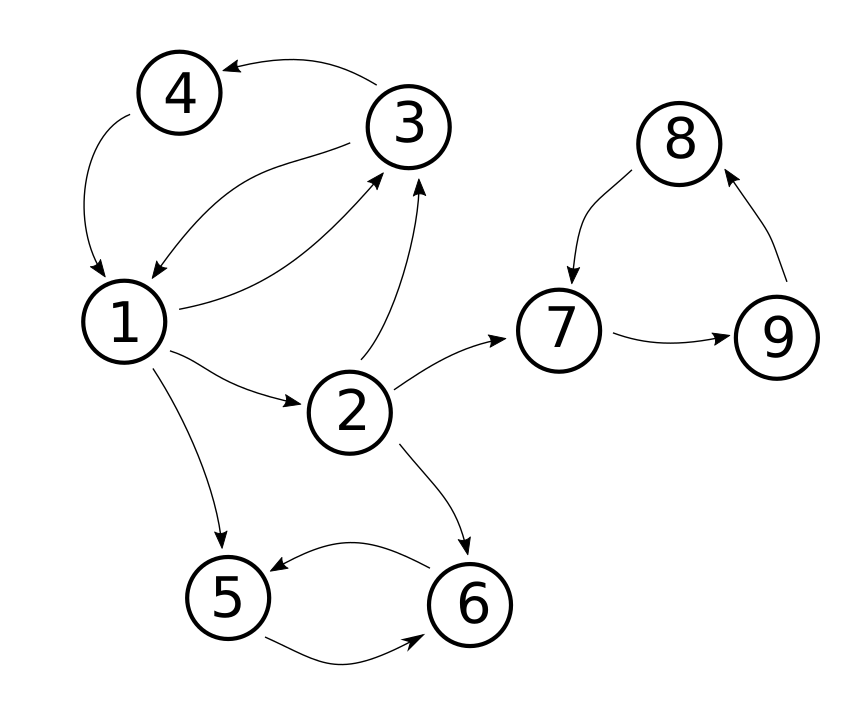
\includegraphics[width=0.6\textwidth]{graph-only.png}
  \caption{Exemple de graphe dirigé}
  \label{fig:normal1}
\end{figure}

Afin de trouver tous les cycles dans ces SSC, l'algorithme de Johnson
est utilisé \cite{johnson}. Contrairement à l'algorithme donné dans le
syllabus du cours, celui-ci nous donne même les cycles imbriqués et
autres.

Finalement, une fois tous les cycles ont été détectés, ils sont
minimisés (simplifiés).

\subsubsection{Étapes}

Par conséquent, la simplification de dettes peut être vu comme un
procès en 3 étapes:

\begin{itemize}
\item \textbf{Isolement des composantes fortement connexes:}

  L'algorithme de Tarjan donné dans le syllabus du cours \cite{syl}
nous suffit pour trouver ces composantes. Le vecteur \texttt{comp}
contient le numéro de composante au quelle les noeuds sont attachés.

Il n'y aura pas de cycles en dehors de (entre) ces composantes.

\begin{figure}[ht!]  \centering
  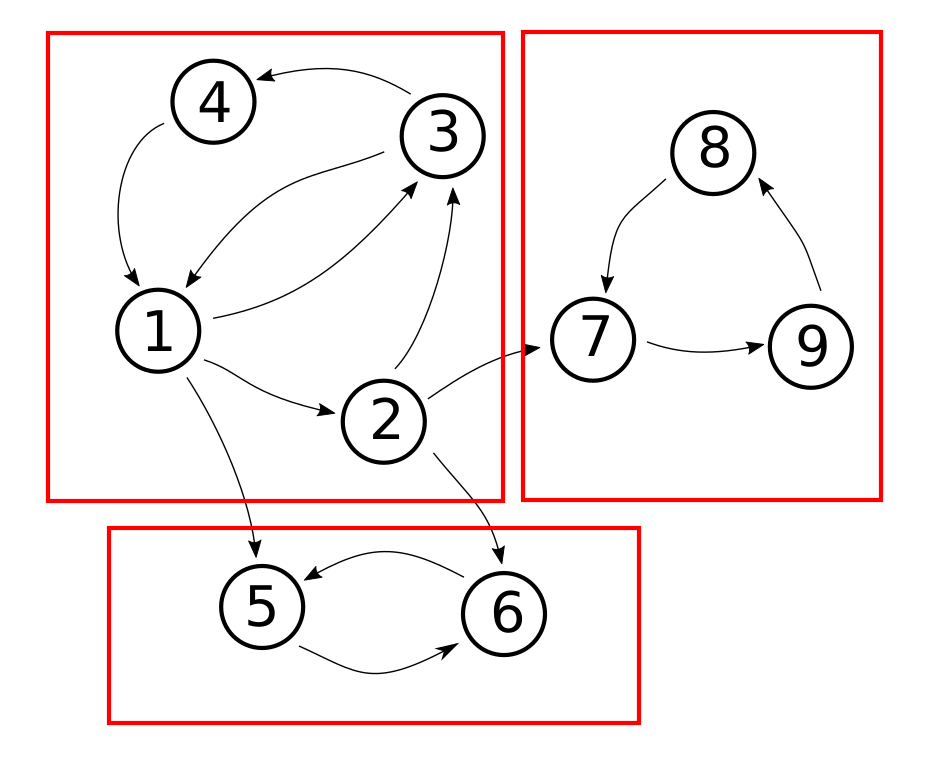
\includegraphics[width=0.6\textwidth]{graph-connexe.png}
  \caption{Composantes fortement connexes dans le graphe}
  \label{fig:normal2}
\end{figure}


\item \textbf{Identification des cycles - Algorithme de Johnson
    \cite{johnson}}

  L'algorithme de Johnson pour trouver les cycles d'un digraphe
  commence par choisir un noeud d'ordre minimale (il doit avoir un
  ordering interne: dans notre cas, la méthode \texttt{\_\_lt\_\_()}
  établit l'ordre en fonction des lettres des noeuds, par example
  \texttt{A\ < \ B}) et tous les noeuds d'un ordre majeur dans
  \textbf{une composante fortement connexe}.

  Ce noeud d'ordre minimale sera retiré du graph une fois traité et le
  noeud de départ sera celui qui a le nouveau ordre minimale.

  On parcourt les voisins de ce noeud \emph{s} et les voisins des
  voisins (en DFS). Pour eviter les cycles dupliqués, un voisin
  \emph{v} est bloqué (on l'ajoute au vecteur \texttt{blocked}) et
  reste bloqué si pour tout chemin de retour de \emph{v} au noeud de
  départ \emph{s}, ceci croisse ou touche notre chemin de parcours
  originel (qu'on a ajouté dans un stack). Quand on arrive de nouveau
  à \emph{s}, un cycle a été trouvé. Si \emph{v} est bloqué ça veut
  dire aussi qu'il ne peut pas être utilisé deux fois dans un même cycle.

Notre pseudo-code est le suivant:

\lstinputlisting{pseudo_code_johnson.txt}

\item \textbf{Simplification des poids des arcs}

  Finalement, le digraphe doit être modifié avec les poids
  reduits. Les étapes sont les suivantes:

  \begin{itemize}
  \item Pour chaque cycle:
    \begin{itemize}
    \item Chercher le poids minimum
    \item Faire la soustraction entre les poids des arcs concernés et
      ce poids minimum
    \end{itemize}
  \end{itemize}
\end{itemize}

\subsubsection{Améliorations}


D'une manière plus générale, cette simplification pourrait être faite
avec une topologie comme celle montrée dans la
fig. \ref{fig:simple2}. Même si le cycle n'existe pas, la personne C
pourrait payer seulement 20 unités (quelque soit la devise) à A et
donner 30 unités a B. Le graphe deviendrait non-dirigé en ce qui
concerne les cycles. Cette capacité n'a pas été implémentée dans ce
projet mais peut être vu comme une amélioration.

\begin{figure}[ht!]  \centering
  \begin{tikzpicture}[->,>=stealth',shorten >=1pt,auto,node
distance=2.5cm, thick,main
node/.style={circle,draw,font=\sffamily\Large\bfseries}]

    \node[main node] (A) {A}; \node[main node] (B) [below left of=A]
{B}; \node[main node] (C) [below right of=A] {C};

    \path[every node/.style={font=\sffamily\small}] (A) edge node
[left] {10} (B) (C) edge node [below] {20} (B) (C) edge node [right]
{30} (A);
  \end{tikzpicture}
  \caption{Exemple simplification de 'transactions'}
  \label{fig:simple2}
\end{figure}

\newpage
\subsection{Identification des communautés}

Cet algorithme permet d'identifier tous les communautés et les
personnes appartenant à chaque une d'entre elles.\par L'algorithme
marche de la façon suivante:\par Il commence par calculer le nombre de
dettes de chaque personne, a fin de minimiser le nombre de fois qu'il
doit parcourir la liste \textit{identifier} pour mettre a jour les
\textit{id}'s.  Il prend la personne qui a plus de dettes et parcourt
tous les noeuds qu'il peut atteindre en les marquant comme visités et
en les attribuent un même \textit{id}.  Si les noeuds n'ont pas encore
tous un \textit{id} (si il existe plus qu'une communauté par exemple),
on prend la personne qui a plus de dettes et qui n'a pas encore été
visité et ont répète le processus.  Dans le cas où on tombe sur une
personne déjà visité, on met à jour les \textit{id}'s.\par À la fin,
tous les noeuds (personnes) d'une même composant connexe (communauté)
auront le même \textit{id} et on peut donc retourner une liste de
communautés.  \lstinputlisting{pseudo_code_community.txt}


\subsection{Identification des hubs sociaux}

L'algorithme d'identification des hubs sociaux permet d'identifier les
points d'articulation d'un graphe tel que sans eux on obtient un plus
grand nombre de composantes connexes d'au moins \textit{n} noeuds.\par
Il commence par appeler une méthode de \textit{graph} pour obtenir un
graphe non dirigé.  Ensuite, il fait un parcours en profondeur,
marquant les noeuds déjà visites avec un id.  Si on trouve un noeud
déjà visité avec un id plus petit, on fait une mise à jour.\par On
sait qu'on a rencontré un point d'articulation quand le \textit{id} de
l'élément \textit{k} est plus petit que le \textit{low} de son
fils. Dans ce cas, l'algorithme stocke la taille de la plus petite
composante connexe créée après la suppression de ce point.
\lstinputlisting{pseudo_code_hub.txt}



\section{Conclusion}

On a travaillé en groupe (binôme). Ensemble, on a écrit l'algorithme
permettant la lecture d'un fichier, la création du graphe aussi bien
que le rapport.\\ Néanmoins, certaines taches ont étés partages:\\
Carlos était en chargé de faire la simplification des dettes, tandis
que Pedro s'a vu responsable de l'identification des communautés et de
l'identification des hubs sociaux.

Avec ce projet on a eu l'opportunité de mettre en pratique une partie
de ce qu'on a vu au cours théorique de M. Frédéric Servais.\par Ça
nous a permis non seulement de milleux comprendre certains algorithmes
mais aussi d'approfondir nos connaissances d'algorithmique en général.

\nocite{*}
\bibliographystyle{plain}
\bibliography{references.bib}


\end{document}